%!TEX root = ../thesis.tex
\newchap{Semileptonic ditop decays}\label{sec:Events}
\vspace{-1cm}
\minitoc


\section{Event signatures}
In this chapter, the $\ttbar \to b\ell\nu \: bcb$ process will be denoted with "signal" or "cb events", while other processes will be referred to as "background".\\
\\
The final state of a signal event consists of one muon or electron, three b jets, one c jet, and missing energy due to the neutrino from the leptonic \PW decay.\\
The invariant mass of one b jet and the c jet should be consistent with the mass of the \PW boson, and, adding another b jet, the invariant mass of the three jets should be consistent with the mass of the top quark.\\
The signal's final state can be mimicked by the following backgrounds.
\begin{itemize}
    \item Semileptonic $\ttbar$ ($\ttbar\to b\ell\nu \: bq\bar{q}$): if one or more jets are mistagged or there are additional heavy flavor jets.\\
    Both the production of additional heavy-flavor jets and the flavor mistagging are suppressed but have to be evaluated.
    \item Dileptonic $\ttbar$ ($\ttbar \to b\bar{\ell}\nu \: \bar{b}\ell\bar{\nu}$): the presence of two leptons in the final states increase the trigger probability, while additional jets can be misidentified as c and b jets originating from the hadronic decay of the W boson.
    \item Dihadronic $\ttbar$ ($\ttbar \to b\bar{q}q \: \bar{b}q\bar{q}$): the lepton that would trigger the event can originate from the semileptonic decay of a meson in the jet if it passes the isolation selections, and the missing b jet can be obtained by mistagging or by additional heavy flavor jets.
    \item W+jets $(\PW \to \ell \nu)$: This process is the one with the largest cross-section but the requirement of three additional b jets and one additional c jet suppresses it significantly.
    \item WW+jets: the semileptonic decay of \PW\PW pairs produced directly by $pp$ collision have required to be produced in association with two additional b jets to present the same signal signatures. Another difference with the signal is the inconsistency of the invariant mass of three jets with the top mass, which, however, is difficult to exploit due to the combinatorial ambiguities and the low tri-jet mass resolution.  
    \item $t\PW+\text{jets}$: it is similar to the $\PW \PW + \text{jets}$ process, with the difference that only one additional b jet, instead of two, is required to match the signal signature.
    \item $tq$ (t-channel): if the     
    top quark decays into a lepton,
    two additional b jets are required to match the signal signatures.   
    Furthermore, if the other quark is not a charm quark, an additional c jet is required too. However, to produce a single top in a t channel, one incoming b quark is needed. Since the b quark production at LHC is mainly due to gluon splitting, the tq (t-channel) is often produced in association with an additional b jet.  
\end{itemize}
The production cross-sections of these processes  at $\sqrt{s}=13\TeV$ with $pp$ collisions are reported in Tab.\ref{tab:cross}


\begin{table}[H]
    \centering
    \fontsize{9.2pt}{9.2pt}\selectfont
    \begin{tabular}{l|cccc|c|c|c|c}
        \toprule
          \multicolumn{1}{c|}{$\mathbf{pp\to}$}&\multicolumn{4}{c|}{$ \mathbf{t\bar{t}}$}&  $ \mathbf{W}$& $ \mathbf{WW}$ & $ \mathbf{tW}$& $ \mathbf{tq}$\\
          &&  &  &  &  &   & & (t-channel)\\
          \midrule
          \multicolumn{1}{c|}{$\mathbf{\sigma (pb)}$}&\multicolumn{4}{c|}{\multirow{2}{*}{$832$}}& \multirow{2}{*}{$190000$} & \multirow{2}{*}{$118$} &  \multirow{2}{*}{79}& \multirow{2}{*}{214} \\
          \multicolumn{1}{c|}{$(13\TeV)$}& &  & & &  &&&\\
          \midrule
          &signal&  semiLept&  diLept&  diHad& Lept &  semiLept & semiLept& Lept\\
          &$(b\ell \nu\: bcb)$&$(b\ell \nu\: b\bar{q}q)$&$(b\bar{\ell} \nu\: \bar{b}\ell \bar{\nu})$&$(\bar{b}\bar{q}q\: b\bar{q}q)$&$(\ell \nu)$&$(\ell \nu \: q\bar{q})$& $(b\ell\nu q \bar{q})$&$(b\ell\nu \: q)$\\
          \midrule
          $\mathcal{BR}$& $3.7 \cdot 10^{-4}$   & 0.439 & 0.106 & 0.455 & 0.326 & 0.439 & 0.439 & 0.326\\
          $ \mathcal{BR}\cdot\mathbf{\sigma} (pb)$& 0.307 & 365 & 88 & 379 & 61000 & 51.8 & 34.7& 69.8 \\
          $\mathcal{BR}\cdot\mathcal{L}_I\mathbf{\sigma} $&$4.2 \cdot 10^4$& $5.0 \cdot 10^7$ &  $1.2 \cdot 10^7$&$5.2 \cdot 10^7$  &  $8.5 \cdot 10^9$ & $7.1 \cdot 10^6$  & $4.8 \cdot 10^6$& $9.6 \cdot 10^{6}$\\
          \bottomrule
    \end{tabular}
    \vspace{0.2cm}
    \caption{Production cross-sections of signal and backgrounds at $\sqrt{s}=13\TeV$. In the first row, there are the production cross-sections from pp collisions at $13 \TeV$, in the following rows there are the respective branching fractions of the different final states, the cross-section of the respective final states, and the total number of events expected in all the Run2, with a total integrated luminosity of $\mathcal{L}_I=138 {fb}^{-1}$}
    \label{tab:cross}
\end{table}

\paragraph*{Analysis strategy}
In the following sections, the selection criteria for physics objects and events are described, defining different signal regions for $\ell=\mu,e$.
Therefore, after reconstructing the kinematics of the events, the signal extraction is performed through a template fit on a NN score, by exploiting multivariate analysis techniques, and also studying the relevant signatures of the events.\\
This work will be conducted only on MC simulations and the observed data will be replaced by the Asimov dataset.



\section{Monte Carlo samples}\label{sec:MC}
The simulation of a hadron-hadron collision relies on different steps and elements \cite{Bierlich2022A8.3}:
\begin{enumerate}
    \item \textbf{PDF set}: The first thing that has to be defined is the parton distribution function of the proton since it defines the initial partons involved in the hard scattering and their fraction of carrying momenta.\\
    In all the simulated samples, the used PDF set is NNPDF3.1 NNLO \cite{TheNNPDFCollaboration2017PartonData}.
    \item \textbf{Generator}: The kinematics of the outgoing particles are based on matrix-element calculated in perturbation theory, using Markov chain Monte Carlo integrators.\\
    The generators that were used to build the MC samples are \MADGRAPH 5, aMC@NLO \cite{Alwall2011MadGraphBeyond}, and \POWHEG 2 \cite{Alioli2010ABOX}, setting $\alpha_s$ to a value of $0.118$ at the Z pole mass.
    All the samples are generated with a different number of additional partons, and with different precision, \ie considering only the leading order (LO) calculations or going forward to the next-to-leading order (NLO) to include virtual corrections.

    \item \textbf{Parton Showers}
    The soft and collinear emission is impossible to be handled at the matrix element level. These effects are reproduced by the parton showers.
    The shower is constructed recursively, increasing the number of partons by one at each step until an energy cutoff at around the hadronization scale is met.\\
    The software that handles the parton showers is \PYTHIA \cite{Bierlich2022A8.3}.

    \item \textbf{Matching}
    The matrix element calculations provide an accurate description of events with well-separated particles in the final state, while the accurate reproduction of collinear and soft emissions is handled by the parton showers.\\
    Matching methods have the scope of improving the accuracy of the description of multijet final states, combining both approaches.\\
    The Monte Carlo samples used in this work are generated using the MLM matching method \cite{Mangano2006MatchingCollisions} if the matrix element calculations are performed at the LO, or using the FxFx method \cite{Frederix2012MergingMCNLO} if the matrix element calculations are performed at the NLO. 

    \item \textbf{Hadronization} The last step is the hadronization that is simulated by exploiting the Lund string model \cite{Andersson1983PartonDynamics} and is handled by \PYTHIA using the \texttt{TuneCP5} set of tuning parameters \cite{Sirunyan2020ExtractionMeasurements}.\\
\end{enumerate}

The reconstruction and the calibration are performed with the \textit{Ultra Legacy 18} (UL18) setting, which reproduces the state of the detector in 2018.\\
The used samples are NanoAOD files \cite{Liu2020TheCMS}, a lightweight data format that consists only of flat ROOT NTuple.
\\
\\
A comparison of all the used samples is reported in Table \ref{tab:samples}.
\begin{table}[H]
    
    \centering
    \fontsize{10.5pt}{10.5pt}\selectfont
    \begin{tabular*}{\linewidth}{@{\extracolsep{\fill}}cccc|c}
    \toprule
    \multirow{2}{*}{\textbf{Dataset}}&\multirow{2}{*}{\textbf{Generator}} & \textbf{Additional} & \multirow{2}{*}{$\mathcal{L}_I^{\text{MC}}/\mathcal{L}_I^{\text{RunII}}$}& \multirow{2}{*}{\textbf{Label}}  \\
    &&\textbf{Partons}& &\\
    \midrule
    \ttbar signal& \MADGRAPH (LO) & \multirow{2}{*}{3} &\multirow{2}{*}{76.5}& $\ell=\mu,e,\tau$  \\
    $(b\ell\nu \: bcb)$ &+\MADSPIN & && signal(Mu,Ele,Tau) \\    
    \midrule
    \ttbar semiLept&\multirow{2}{*}{\POWHEG (NLO)} &\multirow{2}{*}{1}&\multirow{2}{*}{2.24} & $\ell=\mu,e,\tau$   \\
    $(b\ell\nu \: bqq)$ && && TTsemiLept(Mu,Ele,Tau)\\  
    \midrule
    \ttbar diLept&\multirow{2}{*}{\POWHEG (NLO)}  &\multirow{2}{*}{1}&\multirow{2}{*}{1.71} & \multirow{2}{*}{TTdiLept}\\
    $(b\bar{\ell}\nu \:\bar{b}\ell\bar{\nu})$&& &\\
    \midrule
    \ttbar diHad&\multirow{2}{*}{\POWHEG (NLO)} &\multirow{2}{*}{1}&\multirow{2}{*}{0.87} &\multirow{2}{*}{TTdiHad}\\
    $(bq\bar{q}\: \bar{b}q\bar{q})$&& &\\
    \midrule
    W+jets& \MADGRAPH (LO) &\multirow{2}{*}{4}&\multirow{2}{*}{0.01} &\multirow{2}{*}{WJets}\\
    $(W\to\ell\nu)$&+\MADSPIN &&\\
    \midrule
    WW+jets&aMC@NLO (NLO) & \multirow{2}{*}{1} & \multirow{2}{*}{0.56}& \multirow{2}{*}{WWJets}\\
    $\ell \nu \: q\bar{q}$&+\MADSPIN&&\\
    \midrule
    t\PW & \multirow{2}{*}{\POWHEG (NLO)} & \multirow{2}{*}{1} & \multirow{2}{*}{0.16} & \multirow{2}{*}{tW}\\
    $(b\ell\nu q\bar{q})$&&&&\\
    \midrule
    tq (t-channel) & \multirow{2}{*}{\POWHEG (NLO)} &  \multirow{2}{*}{1} & \multirow{2}{*}{0.11} & \multirow{2}{*}{tq}\\
    $b\ell\nu q$&&&&\\

    \bottomrule
    \end{tabular*}
    \caption{MC samples used in this work along with the respective generator used, the number of additional partons set in the generator, and the ratio between the effective luminosity of the MC sample and the integrated luminosity of the RunII. In the "Label" column there are the names that are used as labels in the rest of the thesis.}
    \label{tab:samples}
\end{table}





Simulated events are normalized to
their expected contributions using event weights 
\begin{equation}
    w_{pe}=\frac{\mathcal{L}_I \cdot \sigma_p \cdot w_{e} }{\sum_j w_{j}}
\end{equation}

where $w_{e}$ is the event weight produced by the generator program. The events weights can also multiplied with other corrections needed to improve the agreement between MC and data (\eg flavor corrections, see sec. \ref{sec:jet}).

\section{Physics objects selections}
As already said, the idea of the analysis is to focus on semileptonic (SL) decay to exploit the lepton as a probe, so we are interested in selecting one prompt lepton, along with four jets.
The selection of physics objects is crucial to reject non-prompt leptons that can originate from the semileptonic decays of mesons and jets that can originate from prompt leptons or pile-up.\\
\\
The objects taken into consideration are Particle Flow candidates (see sec. \ref{sec:PF}) and the applied selection cuts are working points (WP) recommended by the CMS Physics Object Groups (POG).\\
Since the signal cross-section is $\sigma_{\text{signal}}\sim 0.3 pb$, the requirements will be minimal to preserve the statistics. 
\subsection{Muons}
\paragraph*{Identification}
The selected muons are PF candidates reconstructed as \emph{Loose Muons} \cite{2018MuonData}, \ie muon candidates that are reconstructed either as a global muon or as an arbitrated tracker muon (aTk Muons)\footnotemark.\\
Furthermore, the selected muons must be in the coverage of the tracker $|\eta|<2.4$, and its transverse momentum has to be $p_T>26\GeV$ to pass the HLT single muon trigger.
\paragraph*{Isolation}
To select prompt muons from the \PW decay, the particle flow isolation criteria are applied.
\footnotetext{Arbitration is the pattern recognition process that assigns each segment uniquely to a single tracker muon.}
\\
The PF isolation is the scalar sum of the transverse momentum of all the charged particles, neutral hadrons, and photons inside a cone of radius $\Delta R<0.4$ around the selected muon, subtracting the contributions that arise from pile-up effects \cite{2018MuonData}.    
\begin{equation}
    \text{Iso}_\mu = \left(\sum_{\text{charged}} p_T+\max\left(0,\sum_{\text{neutral}}E_T+\sum_{\text{photons}}E_T-\sum_{\text{PileUp}}p_T/2\right)\right)\bigg/p_T(\mu)
\end{equation}
The selected working point is the \emph{Loose PF Isolation}: $\text{Iso}_\mu<0.25$, which leads to a muon selection efficiency of $\sim 98\%$ evaluated on $Z \to \mu \bar{\mu}$ samples.


\begin{minipage}{\linewidth}
\begin{minipage}{0.46\linewidth}
\vspace{-1.25cm}
        \begin{table}[H]
        \centering
        %\fontsize{10.2pt}{10.2pt}\selectfont
        \begin{tabular}{c|c}
            \toprule
            \multicolumn{2}{c}{\textbf{Muons}}\\
            \midrule
            \midrule
            \textbf{Muon} & Loose\\
            \textbf{Identification}& (Global/aTk Muon)\\
            \midrule
            $\mathbf{p_T}$& $>26 \GeV$\\
            \midrule
            $\bm{|\eta|}$& $<2.4$ \\
            \midrule
            \multirow{2}{*}{\textbf{PF Isolation}}&Loose\\
            &$(\text{Iso}_\mu<0.25)$\\
            \bottomrule
        \end{tabular}
        \caption{Muons selection cuts.}
    \end{table}
\end{minipage}
\hfill
\begin{minipage}{0.53\linewidth}
      \begin{figure}[H]
            \centering
            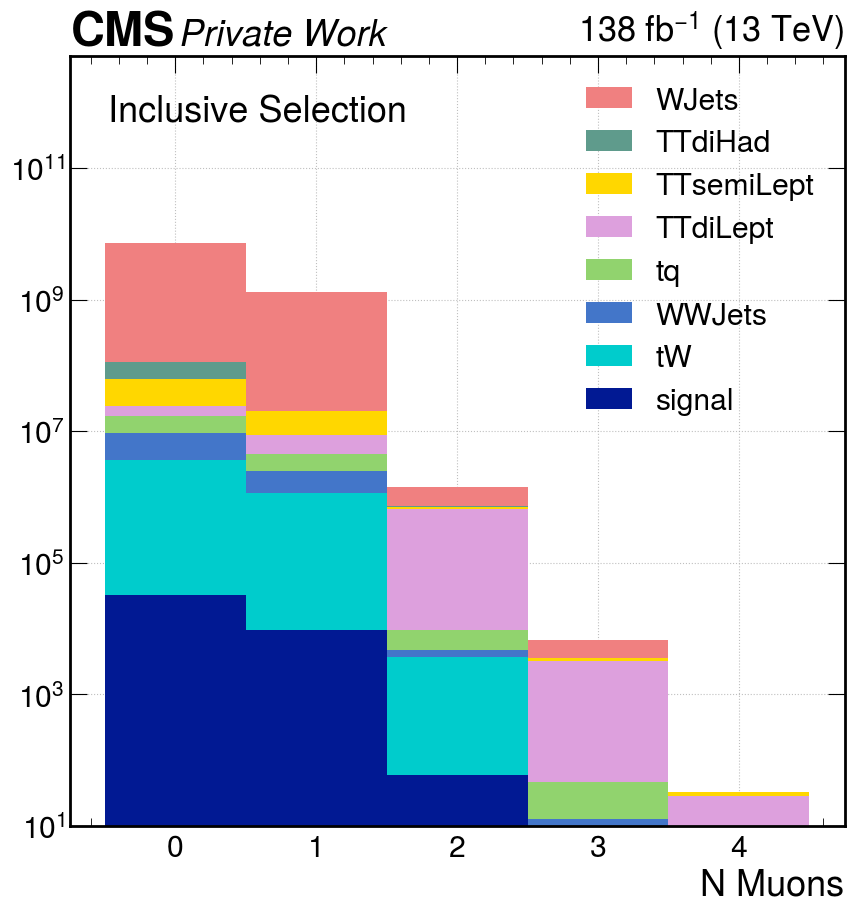
\includegraphics[width=1\linewidth]{fig//chap07-selection/nMuons.png}
            \caption{Distribution on the number of Muons per event.}
            \label{fig:n_mu}
        \end{figure}
\end{minipage}
\end{minipage}


\newpage
\subsection{Electrons}
The selection of electron candidates follows the same principles as the muon selections.
They are required to be into the tracker coverage $|\eta|<2.4$ and its momentum has to be $p_T>30 \GeV$.\\
\\
The identification and isolation of the electron are based on the \emph{medium} working point of \textit{Fall17IsoV2} \cite{2018ElectronConference}, a BDT model which assigns a score to the identification and isolation of the electron, taking as input informations about tracks, calo-clusters, shower shape, the amount of collinear radiation to the electron track, and the PF isolation.\\
\\
The MVA ID is trained on DrellYan+Jets MC samples, with prompt electrons as signal and unmatched plus non-prompt electrons as background, ignoring electrons from tau decays.\\
\\
The medium working point has an overall signal efficiency of $\sim 90\%$ and a background rejection efficiency $>98.5\%$.\\
\begin{minipage}{\linewidth}
    \begin{minipage}{0.53\linewidth}
        \begin{figure}[H]
            \centering
            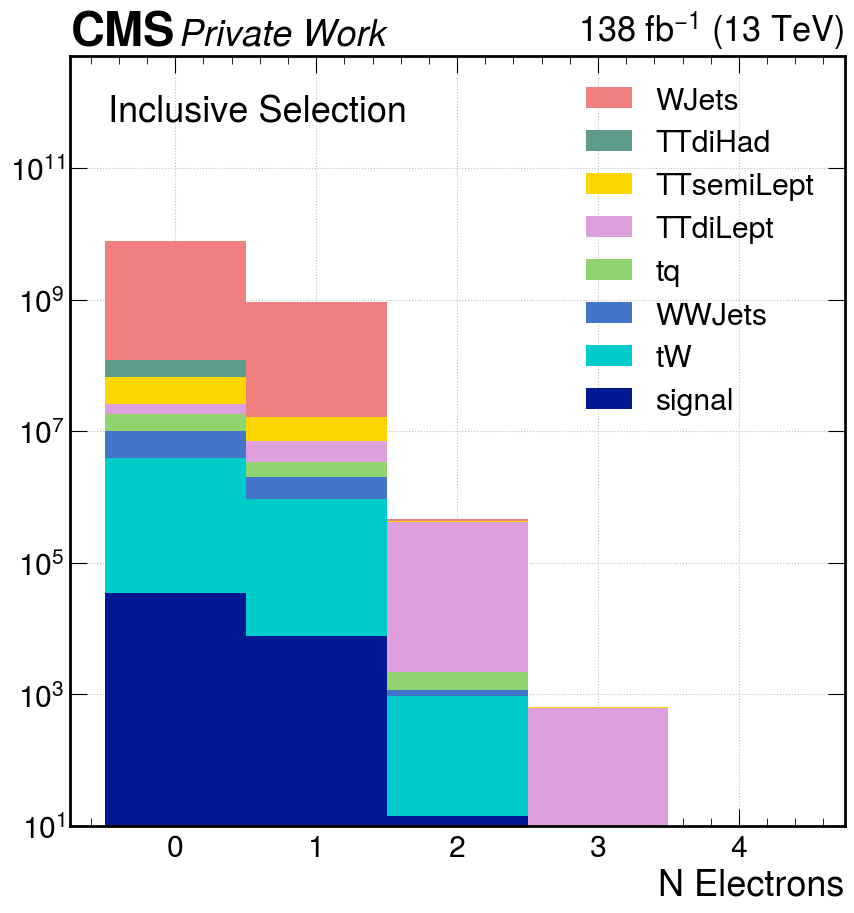
\includegraphics[width=1\linewidth]{fig//chap07-selection/nElectrons.png}
            \caption{Distribution on the number of Electrons per event.}
            \label{fig:n_ele}
        \end{figure}
    \end{minipage}
    \hfill
    \begin{minipage}{0.46\linewidth}
        \vspace{-1.5cm}
        \begin{table}[H]
            \centering
            %\fontsize{13pt}{13pt}\selectfont
            \renewcommand{\arraystretch}{1.48}
            \begin{tabular}{c|c}
                \toprule
                \multicolumn{2}{c}{\textbf{Electrons}}\\
                \midrule
                \midrule
                $\mathbf{p_T}$& $>30 \GeV$\\
                \midrule
                $\bm{|\eta|}$& $<2.4$ \\
                \midrule
                \textbf{$e$ Identification}&Medium WP\\
                \textbf{+ Isolation}&Fall17IsoV2 \\
                &$(\epsilon \sim 90\%)$\\
                \bottomrule
            \end{tabular}
            \caption{Electrons selection cuts.}
        \end{table}      
    \end{minipage}
\end{minipage}


\subsection{Jets}\label{sec:jet}
The jets taken into consideration are the PF AK4 Jet candidates in the calorimeter coverage $|\eta|<4.8$ and with $p_T>20\GeV$.


\paragraph*{Identification}
The jet identification is based on the \emph{Tight jetID} that imposes different requirements on the composition of the jets in different $|\eta|$ regions.\\
The requirements are listed in Tab.\ref{tab:jet_id}

\begin{table}[H]
    \centering
    \fontsize{11pt}{11pt}\selectfont
    \begin{tabular}{l|c|c|c|c}
        \toprule
         \multicolumn{1}{c|}{$\bm{|\eta|\in}$}&  $[0,2.6]$& $[2.6,2.7]$ & $[2.7,3.0]$ & $[3.0,5.0]$\\
         \midrule
         \textbf{Neutral Hadron Fraction} & $<0.90$ &  $<0.90$ & - & $>0.20$\\
         \midrule
         \textbf{Neutral EM Fraction} & $<0.90$ & $<0.99$ & $\in[0.02,99]$ & $<0.90$\\
         \midrule
         \textbf{Number of Constituents } & $>1$ & - & - &  -\\
         \midrule
         \textbf{Charged Hadron Fraction} & $>0$ & - & - & -\\
         \midrule
         \textbf{Charged Multiplicity} & $>0$ & $>0$ & - & -\\
         \midrule
         \textbf{Number of Neutral Particles}& - & - & $>2$ & $>10$\\
         \bottomrule
    \end{tabular}
    \caption{Tight jet identification requirements.}
    \label{tab:jet_id}
\end{table}
The efficiency of the tight Id working point is $\epsilon>99\%$, whereas the background rejection is $>98\%$. 
\paragraph*{Cross-cleaning} 
Since the leptons are included in the jet clustering process, to avoid considering the leading lepton as an additional jet, a simple $\Delta R$ matching is performed. If the jet axis and the leading lepton are separated less than $\Delta R<0.4$, the jet is removed. 

\paragraph*{Pile-up rejection}
The identification of jets from pile-up relies on three types of properties of the jets:
\begin{itemize}
    \item  In the tracker acceptance, the tracks associated with the jets can be used to match the jet with the primary interaction vertex.
    \item The shape of the calorimetric deposit is different in case of overlap of multiple interactions.
    \item The objects' multiplicity.
\end{itemize}


\begin{minipage}{\linewidth}
    \begin{minipage}{0.35\linewidth}
    
        The identification of jets from pile-up is done exploiting the \emph{Jet puId},
        a BDT model score \cite{CMSCollaboration2020PileupData}. Its inputs are listed in Tab \ref{tab:puId_inputs}.\\
        \\
        This BDT is trained on DrellYan+Jets MC samples with jets of $p_T<50\GeV$, where there is the highest composition of PU jets.\\
        
    \end{minipage}
    \hfill
    \begin{minipage}{0.625\linewidth}
    \vspace{-1.65cm}
    \begin{figure}[H]
        \centering
        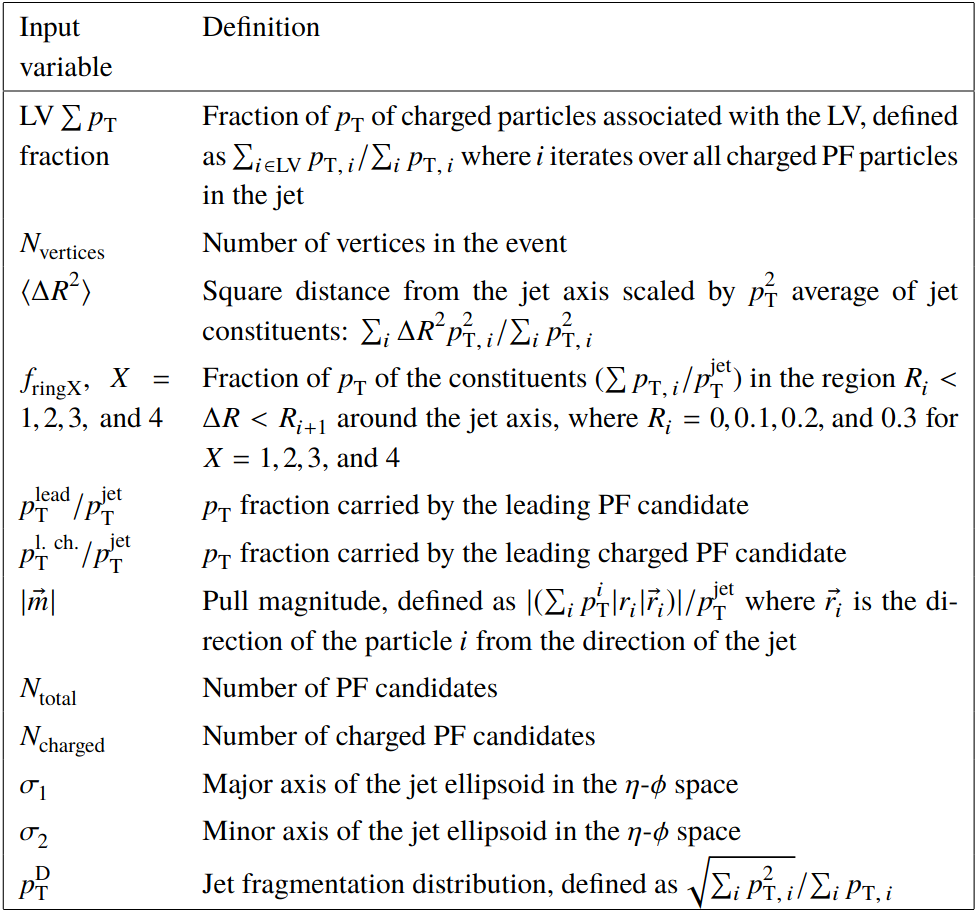
\includegraphics[width=\linewidth]{fig//chap07-selection/puid_bdt.png}
        \captionof{table}{PuID BDT input variables \cite{CMSCollaboration2020PileupData}.}
        \label{tab:puId_inputs}
    \end{figure}
        \vspace{0.1cm}
    \end{minipage}
\end{minipage}
The chosen working point is the \emph{Loose puId}, which corresponds to 99\%  efficiency for prompt jets with $|\eta| < 2.5$ and 95\% efficiency for prompt jets with $|\eta| > 2.5$.
\paragraph*{Jet energy scale corrections}
To allow a proper mapping of the energy of the reconstructed jet to the truth particle-level jet energy, a set of jet energy corrections is applied.\\
\\
In CMS, the jet energy scale corrections are separated into different steps applied sequentially and in a fixed order.\\
Each correction takes care of a different effect and consists of a rescaling of the jet four-vector \cite{2021Jet13TeV}.

\begin{figure}[H]
    \centering
    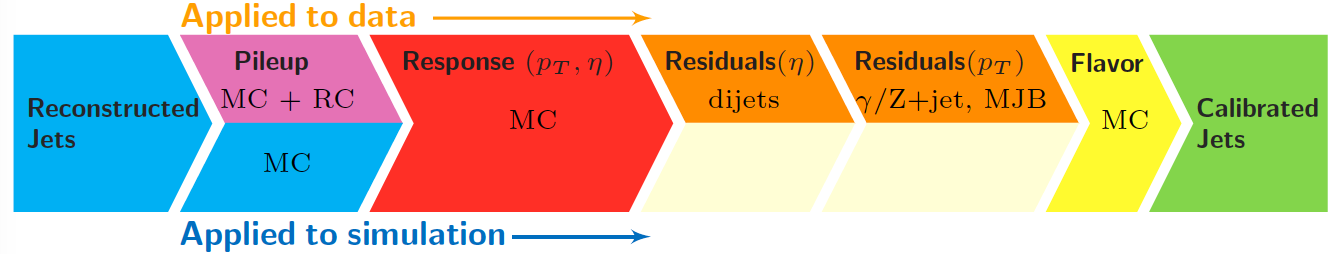
\includegraphics[width=\linewidth]{fig//chap07-selection/JEC.png}
    \caption{Jet energy scale correction chain.}
    \label{fig:jerc}
\end{figure}
\begin{enumerate}
    \item \textbf{L1 Pile-Up}: remove the energy coming from pileup events, removing any dependence on the luminosity.\\
    The pileup corrections are determined from simulated QCD dijet events with and without pileup overlay.
    \item \textbf{L2L3 MC-truth corrections}: this correction has the scope to improve the accordance between the reconstructed jet energy and the particle-level energy, and to make the response of the jet energy uniform in $p_T$ and $\eta$. The related scale factors are evaluated on QCD dijet samples.
\end{enumerate}
The pile-up and MC-truth corrections are applied both on MC and data, while additional residual corrections are applied only on data: they are meant to correct differences of the order of 1\% within jet response in data and MC.

A summary of the jet energy corrections chain is shown in \Fig{fig:jerc}.

\paragraph*{Jet energy resolution corrections}
The jet momentum resolution is different in the data with respect to the simulation. To replicate the resolution observed in the data, the jets' four vectors are rescaled in a procedure called \emph{smearing} \cite{2021Jet13TeV}:\\
if a reconstructed jet and a jet at the generator level (GenJet) are matched through the relation $\Delta R(\text{Jet,GenJet})<0.2$ and $|p_T-p_T^{\text{Gen}}|<3\sigma p_T$, the jet four-vector is scaled by a factor
\begin{equation}
    f=1+\textit{SF}\:\frac{p_T-p_T^{\text{Gen}}}{p_T}
\end{equation}
where $\sigma$ is the jet energy resolution measured with data, and SF is the scale factors that depend on the $\eta$ region in which the jet belongs.
Otherwise, if there is not any match between the jet and the genjets, a random Gaussian smearing is applied.


\paragraph*{Flavor tagging corrections}
The distribution shapes of the \DeepJet discriminators are another element that shows discrepancies between data and simulated samples.\\
To address this problem the events are reweighted:
a weight is applied to each selected jet and an event weight is defined as the product of all the jet weights inside the event.\\
The event weights obtained from these corrections are then multiplied by the event weights provided by the generator program, as already explained in sec. \ref{sec:MC}. 
\\
\\
In this work, the applied corrections are the ones related to the b tagging and to the c tagging.\\
These scale factors are computed through an iterative tag-and-probe procedure \cite{2021B-tagging2018.}, in different bins of $\eta$,$p_T$, and \DeepJet score to compute simultaneously SF for both heavy and light flavor jets.
\begin{itemize}
    \item For heavy-flavor jets, dileptonic $\ttbar$ events are exploited, using one b jet that passes the medium working point as a tag and the second b jet as a probe.
    \item For light jets, Z+jets dileptonic samples are used, using a b tag loose working point as a veto to select the tag jet.
\end{itemize}
The procedure to obtain SFs related to the c-tagging is similar, using W+c samples, but for them, the binning depends both on the CvB and CvL discriminators defined as
\begin{equation}
\begin{aligned}
     \text{CvL} &= \frac{P(c)}{P(c) + P(udsg)}\\
     \text{CvB} &= \frac{P(c)}{P(c) + P(b)} \cdot P(b) 
\end{aligned}
\end{equation}
where $P(b), P(c),$ and $P(udsg)$ are the b,c, and light flavor \DeepJet scores.



\begin{minipage}{\linewidth}
\begin{minipage}{0.53\linewidth}
      \begin{figure}[H]
            \centering
            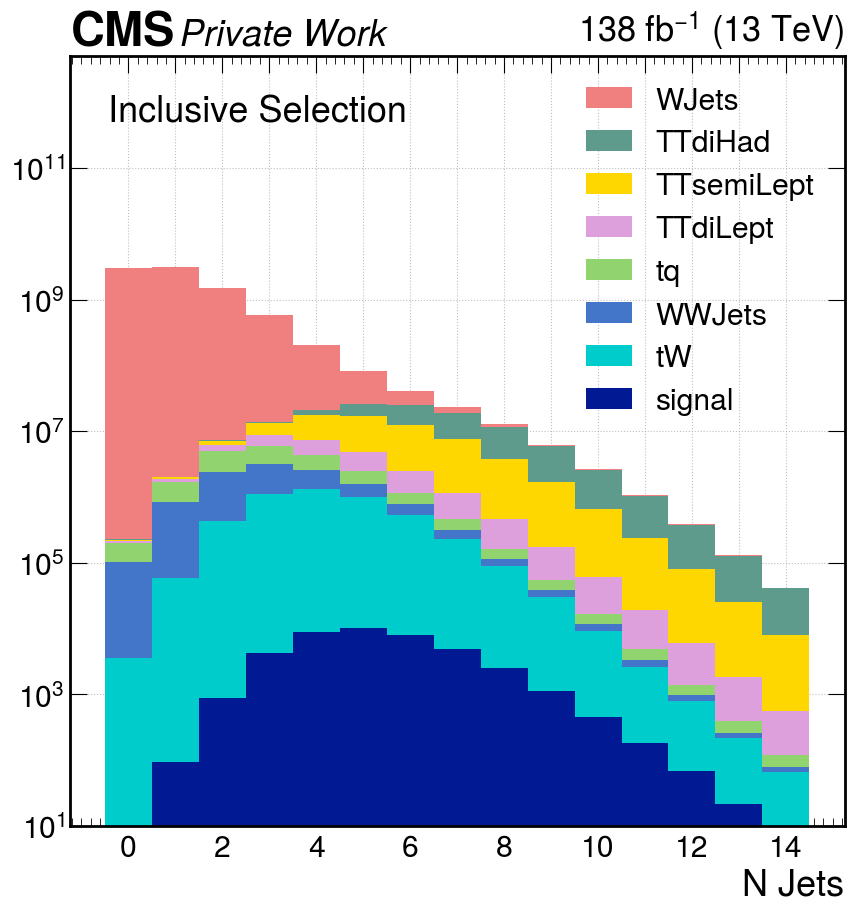
\includegraphics[width=1\linewidth]{fig//chap07-selection/nJet.png}
            \caption{Distribution on the number of Jets per event.}
            \label{fig:n_jet}
        \end{figure}
\end{minipage}
\hfill
\begin{minipage}{0.46\linewidth}
\vspace{-1.25cm}
\begin{table}[H]
    \centering
    \begin{tabular}{c|c}
        \toprule
        \multicolumn{2}{c}{\textbf{Jets}}\\
        \midrule
        \midrule
        
        $\mathbf{p_T}$& $>20 \GeV$\\
        \midrule
        $\bm{|\eta|}$& $<4.8$ \\
        \midrule
        \textbf{Identification} & Tight\\
        \midrule
        \multirow{2}{*}{\textbf{Isolation}} & Lead. Lept. \\
        &$\Delta R>0.4$ matching\\
        \midrule
        \textbf{Pile-up Id} & Loose  $(\epsilon\sim99\%)$ \\
        \bottomrule
    \end{tabular}
    \caption{Jets selection cuts.}
\end{table}
\end{minipage}   
\end{minipage}

 
\newpage
\section{Event selections}
As already discussed, the chosen event selection is minimal to avoid large losses in signal acceptance efficiency.\\ 
The signal events are targeted in two different final states, defined by the flavor of the lepton used as a probe, so after the physics objects selection and the requirement of the presence of at least 4 jets, two different channels are defined: a Muon channel that contains events with at least one selected muon, and an Electron channel that contains events with at least one selected electron.

\vspace{1.25cm}
\begin{figure}[H]
     \centering
     \begin{subfigure}{0.42\linewidth}
         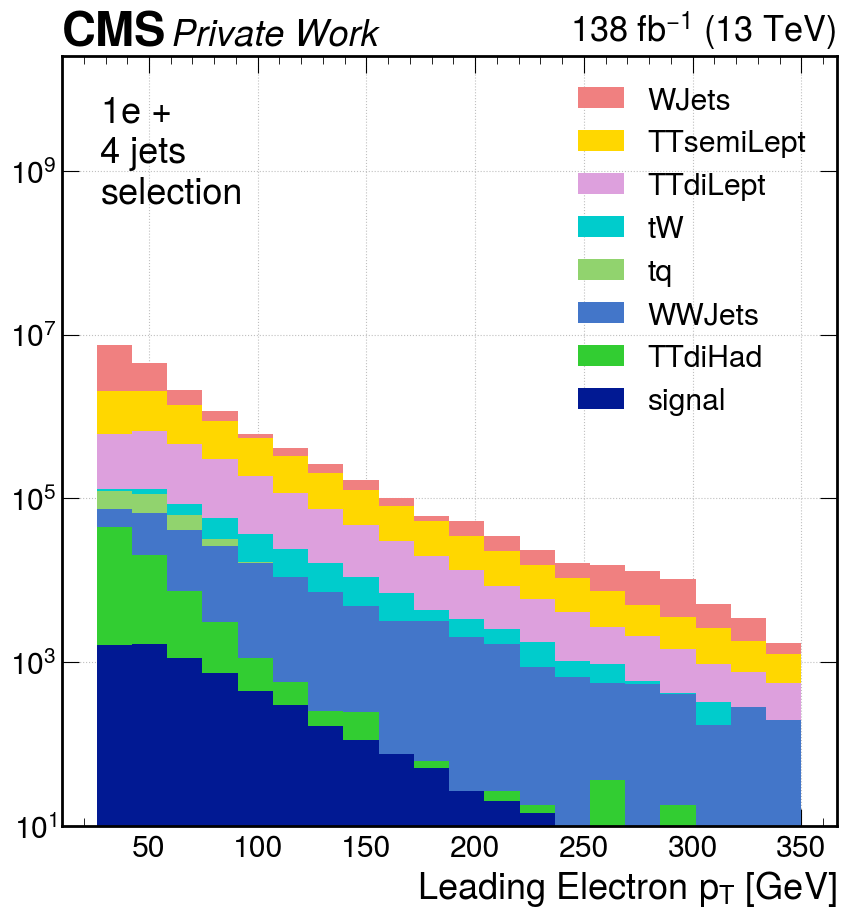
\includegraphics[width=\linewidth]{fig//chap07-selection/selection/Leading_Electron_pt.png}
         \caption{Leading electron}
     \end{subfigure}
     \begin{subfigure}{0.42\linewidth}
        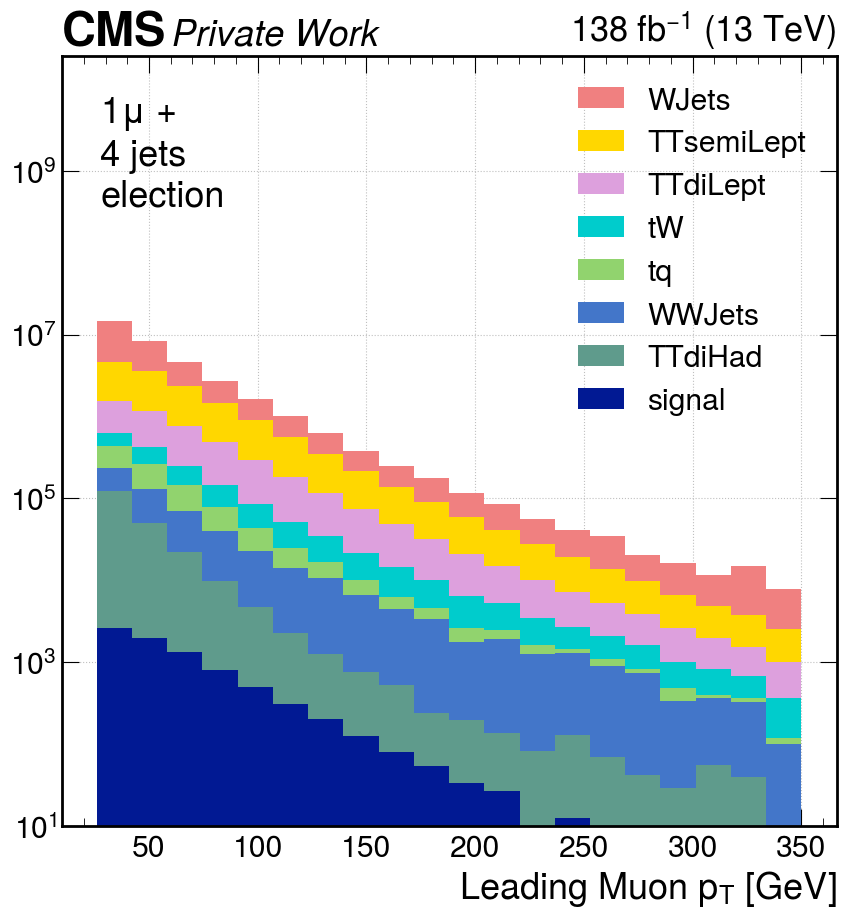
\includegraphics[width=\linewidth]{fig//chap07-selection/selection/Leading_Muon_pt.png}
         \caption{Leading muon}
     \end{subfigure}
     \begin{subfigure}{0.42\linewidth}
        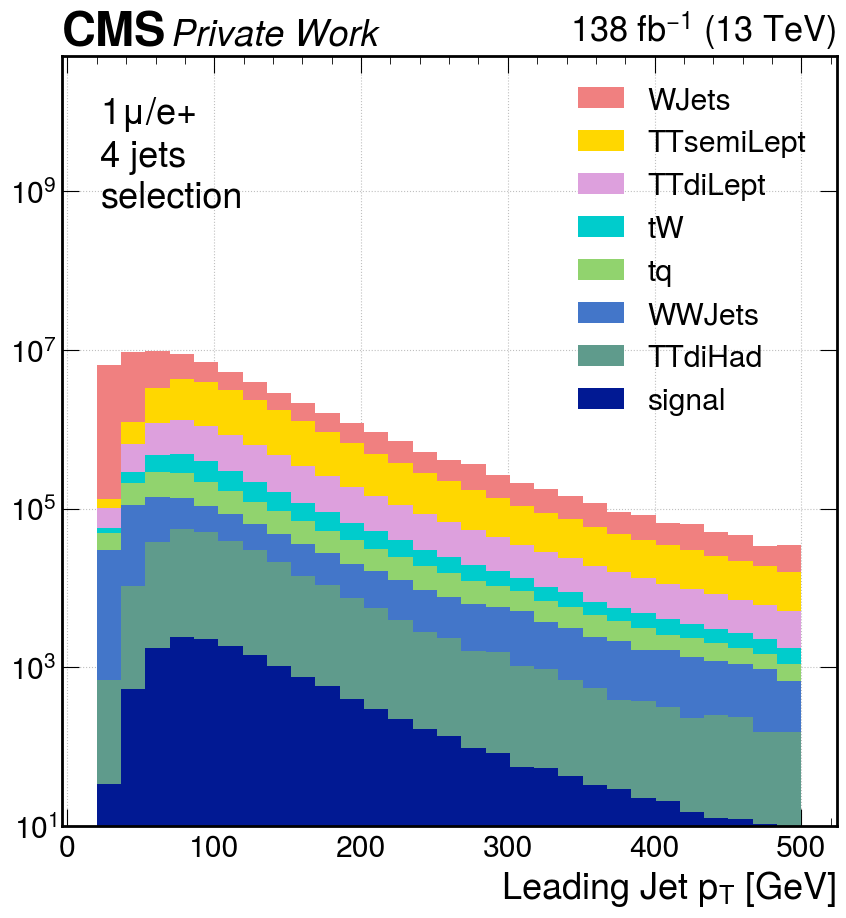
\includegraphics[width=\linewidth]{fig//chap07-selection/selection/Leading_Jet_pt.png}
         \caption{Leading Jet}
     \end{subfigure}
    \begin{subfigure}{0.42\linewidth}
        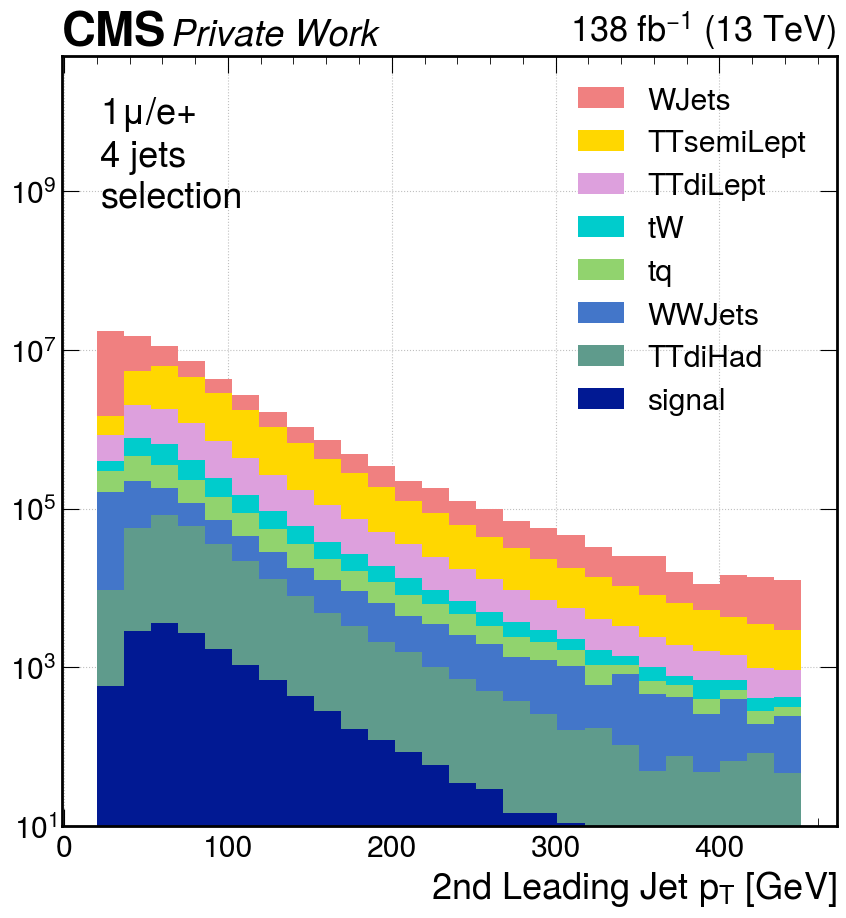
\includegraphics[width=\linewidth]{fig//chap07-selection/selection/Second_Leading_Jet_pt.png}
         \caption{Second Leading Jet}
     \end{subfigure}
\end{figure}
\vspace{-0.5cm}
\begin{figure}[H]
    \ContinuedFloat
    \centering
    \begin{subfigure}{0.42\linewidth}
        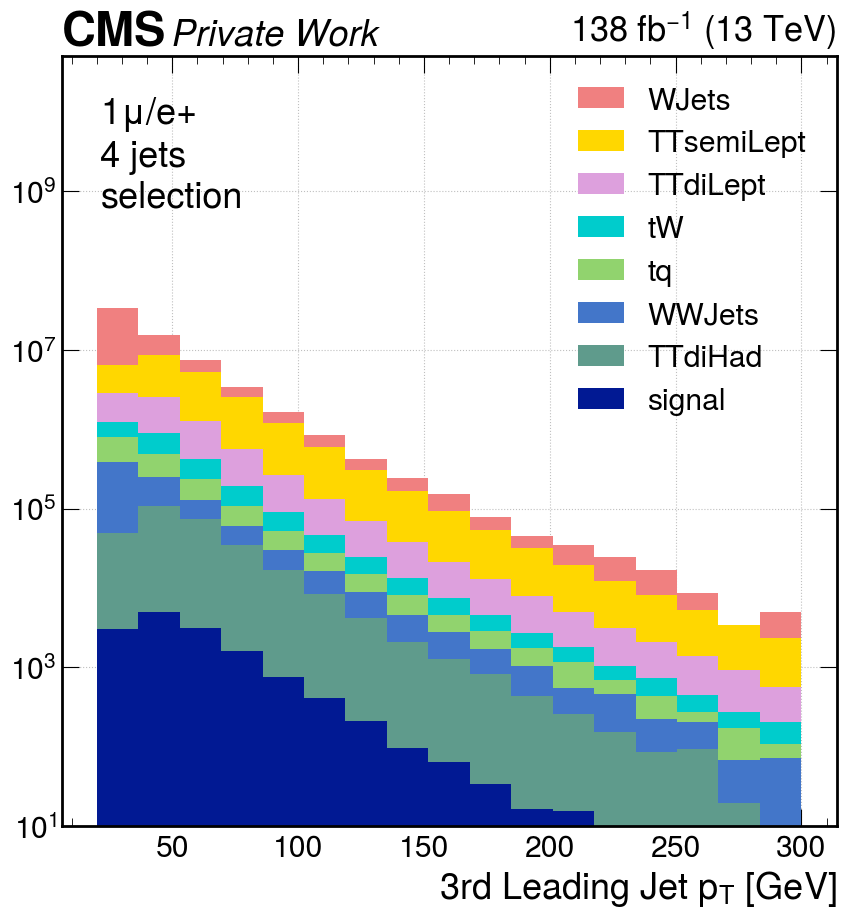
\includegraphics[width=\linewidth]{fig//chap07-selection/selection/Third_Leading_Jet_pt.png}
         \caption{Third Leading Jet}
     \end{subfigure}
    \begin{subfigure}{0.42\linewidth}
        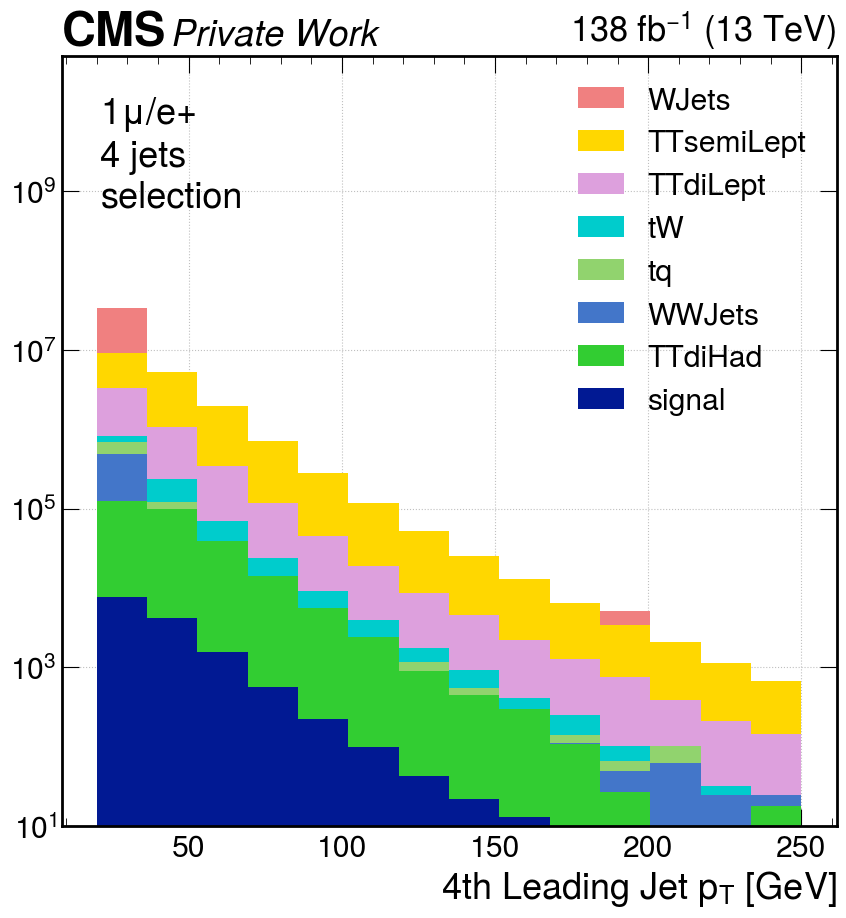
\includegraphics[width=\linewidth]{fig//chap07-selection/selection/Fourth_Leading_Jet_pt.png}
         \caption{Fourth Leading Jet}
     \end{subfigure}
        \caption{$p_T$ distributions after the object selection and the $1e/\mu$ + 4 jets requirements.}
\end{figure}
\vspace{-0.5cm}
An additional selection on the most b-tagged jet is imposed using the medium working point suggested by the BTag\&Vertexing (BTV) POG.\\
The cumulative efficiencies of each cut are described in Tab.\ref{tab:event_selection} and the final event counts normalized with the RunII luminosity and the respective cross-sections in \Fig{fig:event_selection}
\begin{table}[H]
    \centering
    \fontsize{11.pt}{11.pt}\selectfont
    \begin{tabular}{l|ccc||ccc}
        \toprule
         &  \multicolumn{3}{c||}{\textbf{Muons}} &\multicolumn{3}{c}{\textbf{Electrons}} \\
         \midrule
         \midrule
         Cumulative& \multirow{2}{*}{$\bm{\geq1 \mu}$} & \multirow{2}{*}{$\bm{\geq4}$ \textbf{Jets}} & $\bm{\max({\textbf{btag}})}$& \multirow{2}{*}{$\bm{\geq1e}$} & \multirow{2}{*}{$\bm{\geq4}$ \textbf{Jets}} & $\bm{\max({\textbf{btag}})}$\\
         efficiencies&&&$\bm{>0.27}$&&&$\bm{>0.27}$\\
         \midrule
         \textbf{signalMu}& $64.1\%$ & $53.5\%$ & $51.8\%$ &0.22\% & 0.18\% & 0.16\%\\
         \midrule
         \textbf{signalEle}& 0.65\% & 0.50\% & 0.46\% & 52.3\% & 43.5\% & 42.1\% \\
         \midrule
         \textbf{signalTau}& 4.86\% & 3.95\% & 3.80\% & 3.37\% & 2.79\% & 2.70\%\\
         \midrule
         \textbf{TTsemiLeptMu}& 63.6\% & 54.0\% & 49.8\% & 0.15\% & 0.12\% & 0.09\% \\
         \midrule
         \textbf{TTsemiLeptEle}& 0.48\% & 0.39\% & 0.30\% & 51.9\% & 45.6\% & 41.7\% \\
         \midrule
         \textbf{TTsemiLeptTau}&4.59\%  & 3.84\% & 3.48\% &3.24\% &2.82\% &2.58\%\\
         \midrule
         \textbf{TTdiLept}& 40.9\% & 27.4\% & 25.3\% & 33.8\% &22.7\% &20.9\% \\
         \midrule
         \textbf{TTdiHad}& 0.45\%  & 0.40\% & 0.31\% & 0.16\% &0.15\% &0.12\% \\
         \midrule
         \textbf{WJets Lept}& 15.0\% & 0.24\% & 0.03\% & 10.6\% & 0.20\% &0.03\%\\
         \midrule
         \textbf{WWJets SL}& 19.4\% & 5.52\% & 0.81\% & 15.3\% & 4.42\% & 0.64\% \\
         \midrule
         \textbf{tW SL}& 26.7\% & 13.4\%  & 11.2\% & 21.7\% &10.8\% &9.0\%  \\
         \midrule
         \textbf{tq Lept}& 20.5\%  & 5.13\% & 4.27\% & 15.0\% & 3.83\% &3.18\% \\
         \bottomrule
    \end{tabular}
    \caption{Cumulative efficiencies of the selections in the Muons and Electrons channel after the physics objects selection}
    \label{tab:event_selection}
\end{table}
\vspace{-0.5cm}
The main background contribution in each channel is from the \ttbar semileptonic decay, which is 3 orders of magnitude greater than the signal.
Another significant contribution is from the \ttbar dileptonic (DL) process. The contribution from the WW+Jets process is two orders of magnitude smaller than \ttbar SL and \ttbar DL processes, while the remaining processes' contribution is one order of magnitude smaller than the leading backgrounds. 

\begin{figure}[H]
     \centering
     \begin{subfigure}{0.42\linewidth}
         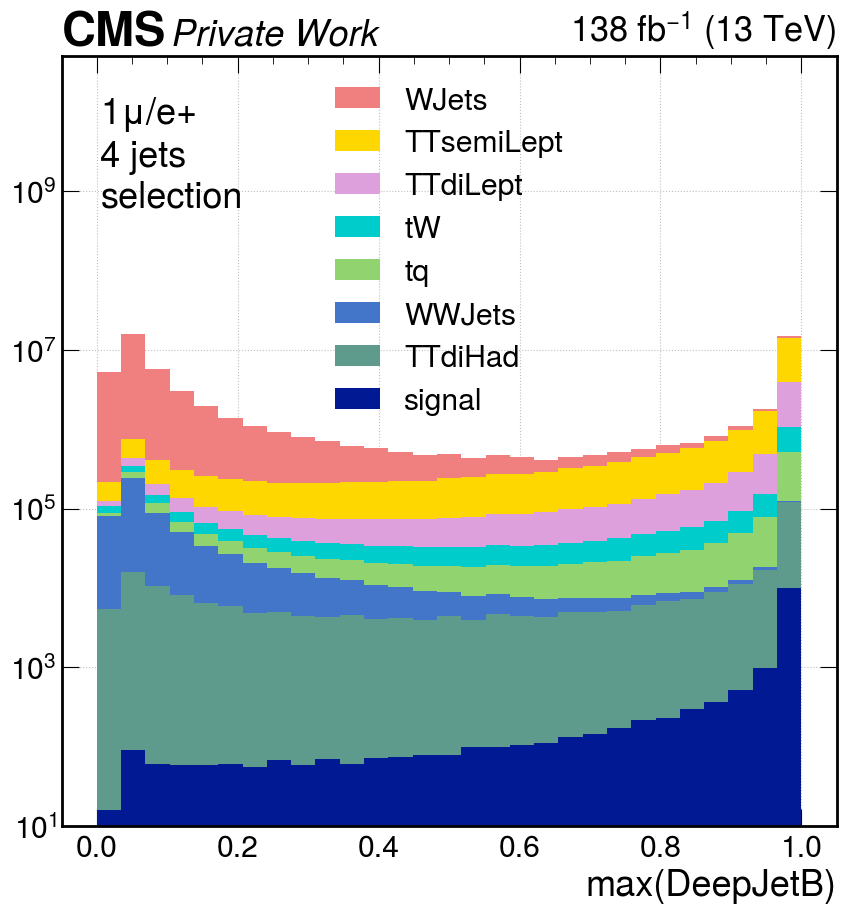
\includegraphics[width=\linewidth]{fig//chap07-selection/btag/Max_DeepJetB.png}
         \caption{Max \DeepJet B}
     \end{subfigure}
    \begin{subfigure}{0.42\linewidth}
         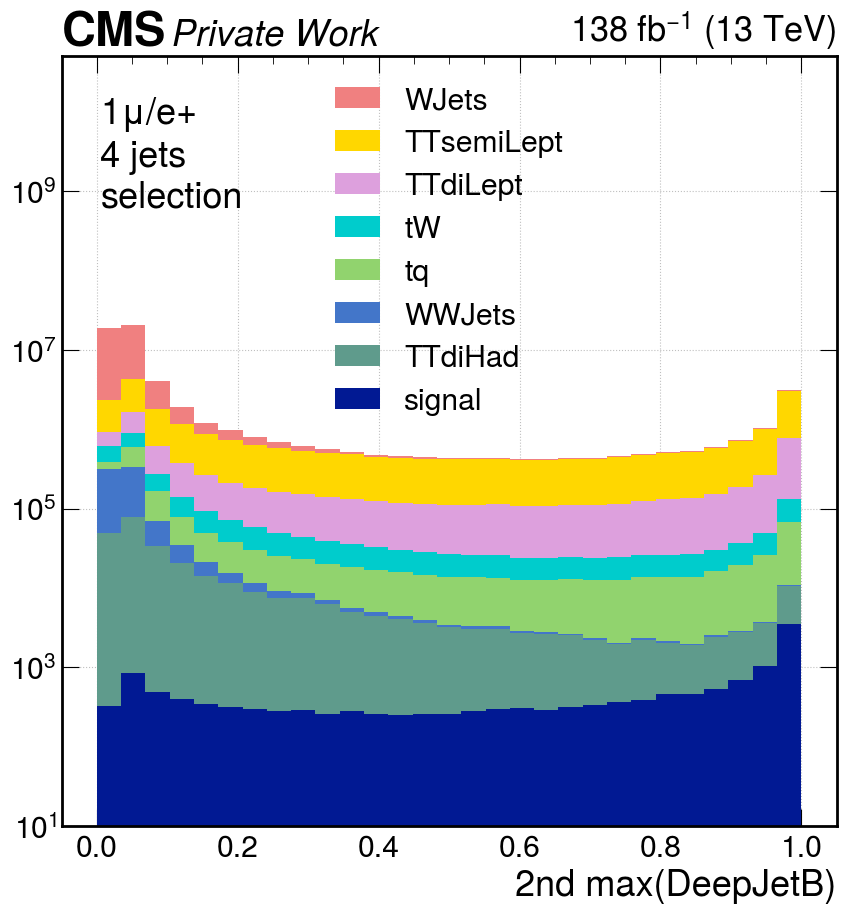
\includegraphics[width=\linewidth]{fig//chap07-selection/btag/Second_Max_DeepJetB.png}
         \caption{Second Max \DeepJet B}
     \end{subfigure}
    \begin{subfigure}{0.42\linewidth}
         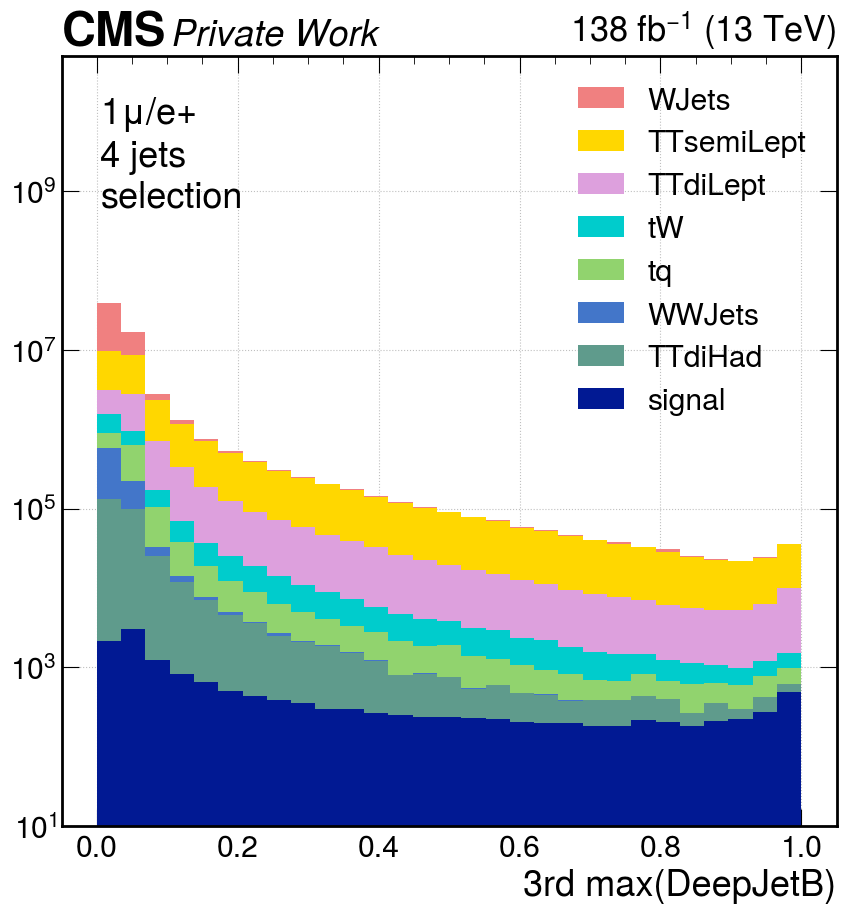
\includegraphics[width=\linewidth]{fig//chap07-selection/btag/Third_Max_DeepJetB.png}
         \caption{Third Max \DeepJet B}
     \end{subfigure}
    \begin{subfigure}{0.42\linewidth}
         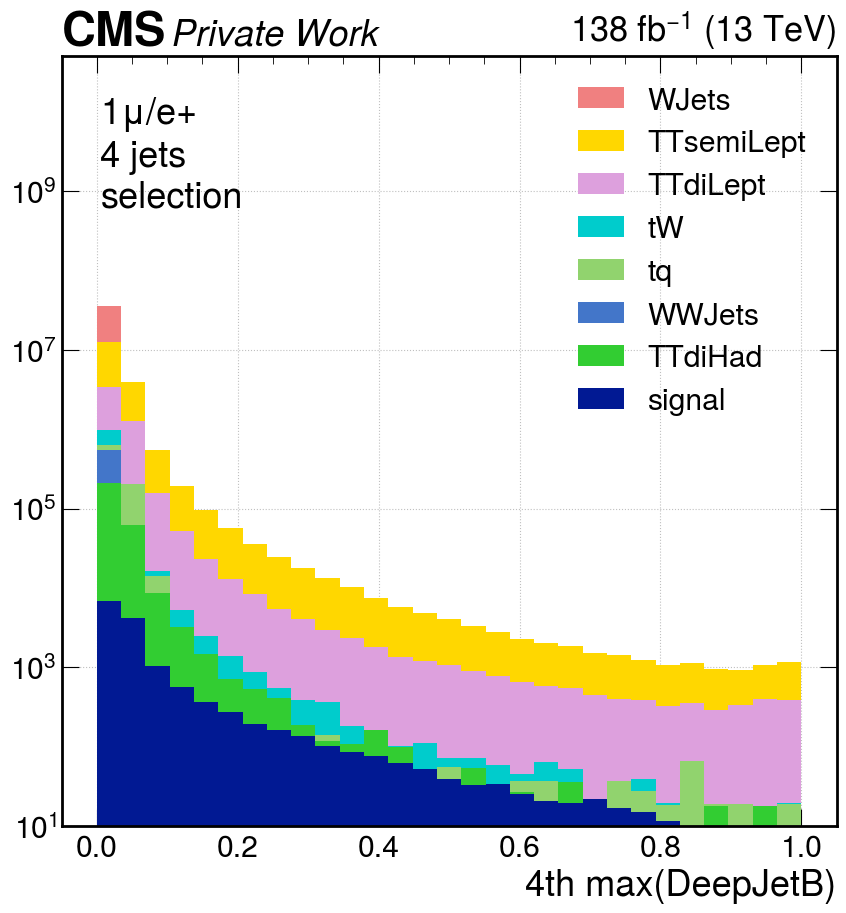
\includegraphics[width=\linewidth]{fig//chap07-selection/btag/Fourth_Max_DeepJetB.png}
         \caption{Fourth Max \DeepJet B}
     \end{subfigure}
          \begin{subfigure}{0.42\linewidth}
         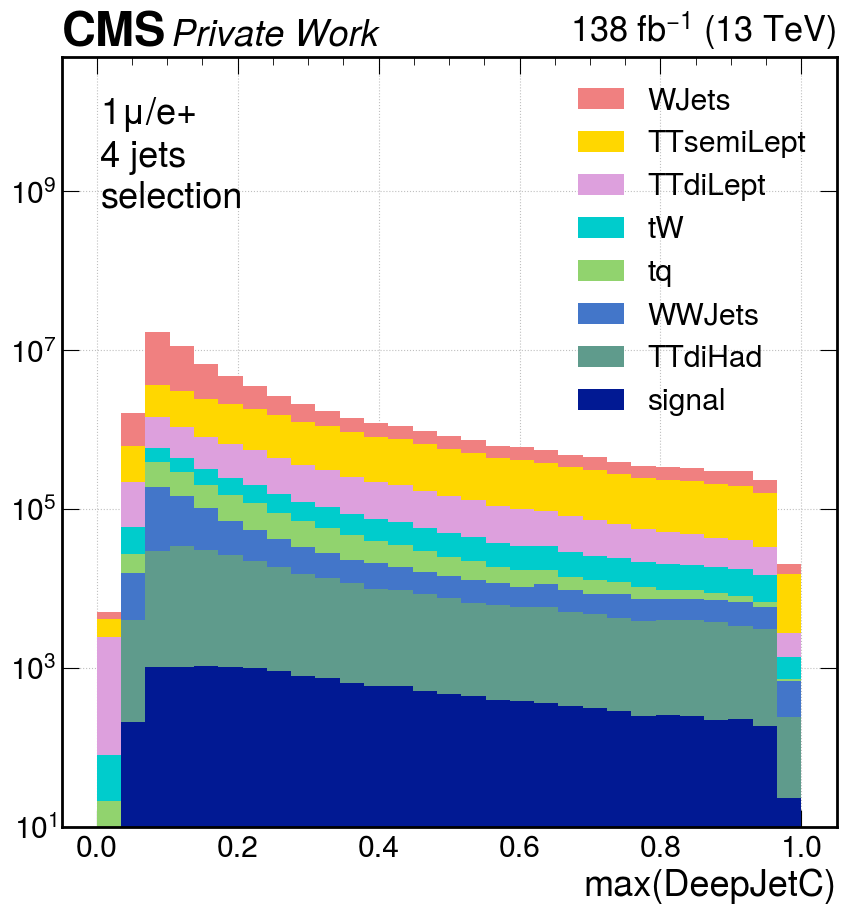
\includegraphics[width=\linewidth]{fig//chap07-selection/btag/Max_DeepJetC.png}
         \caption{Max \DeepJet C}
     \end{subfigure}
    \begin{subfigure}{0.42\linewidth}
         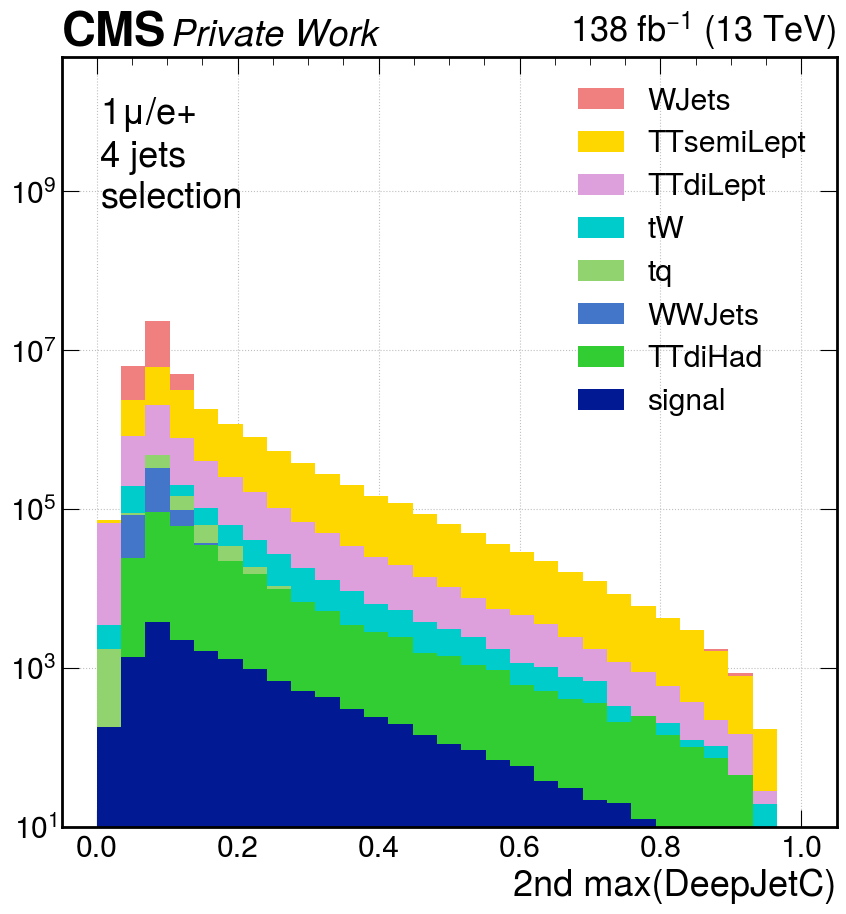
\includegraphics[width=\linewidth]{fig//chap07-selection/btag/Second_Max_DeepJetC.png}
         \caption{Second Max \DeepJet C}
     \end{subfigure}
     \caption{B-tag and c-tag score distributions after the object selection and the 1 lepton + 4 jets requirements.}

\end{figure}
\begin{figure}[H]
     \centering
     \begin{subfigure}[t]{\linewidth}
         \centering
         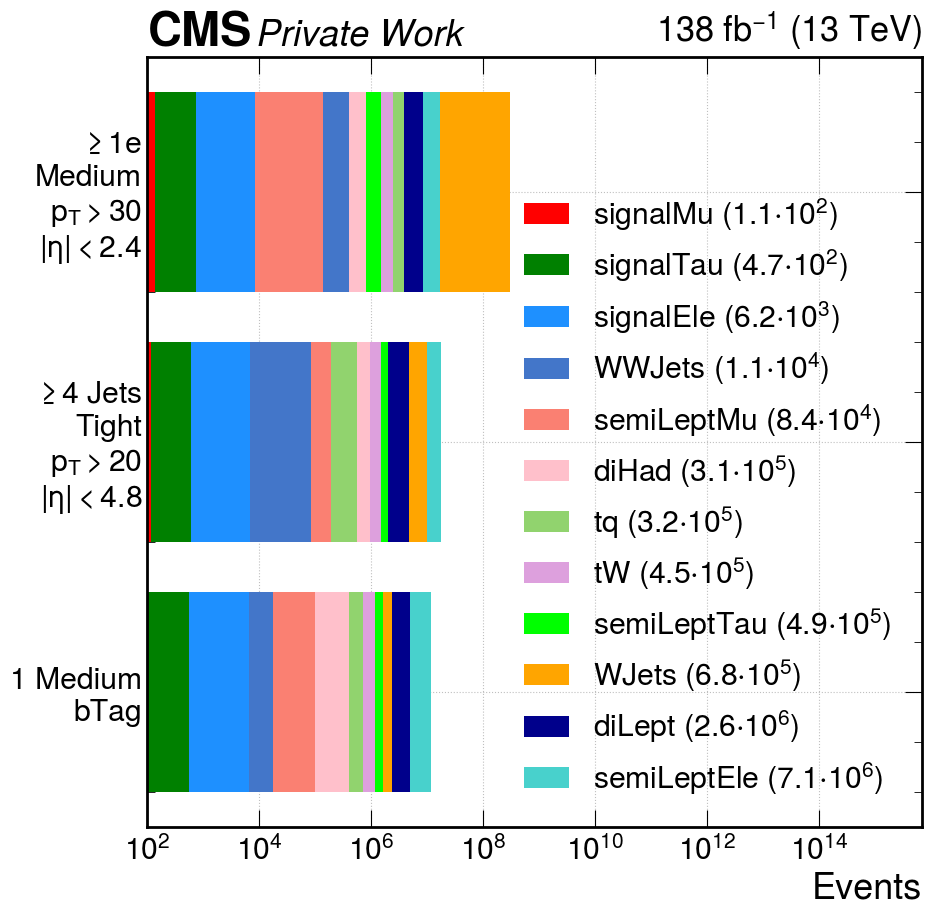
\includegraphics[width=\linewidth]{fig//chap07-selection/ele_selection.png}
         \caption{\textbf{Electrons channel}}

     \end{subfigure}
     
     \vspace{1cm}
     \begin{subfigure}[b]{\linewidth}
         \centering
        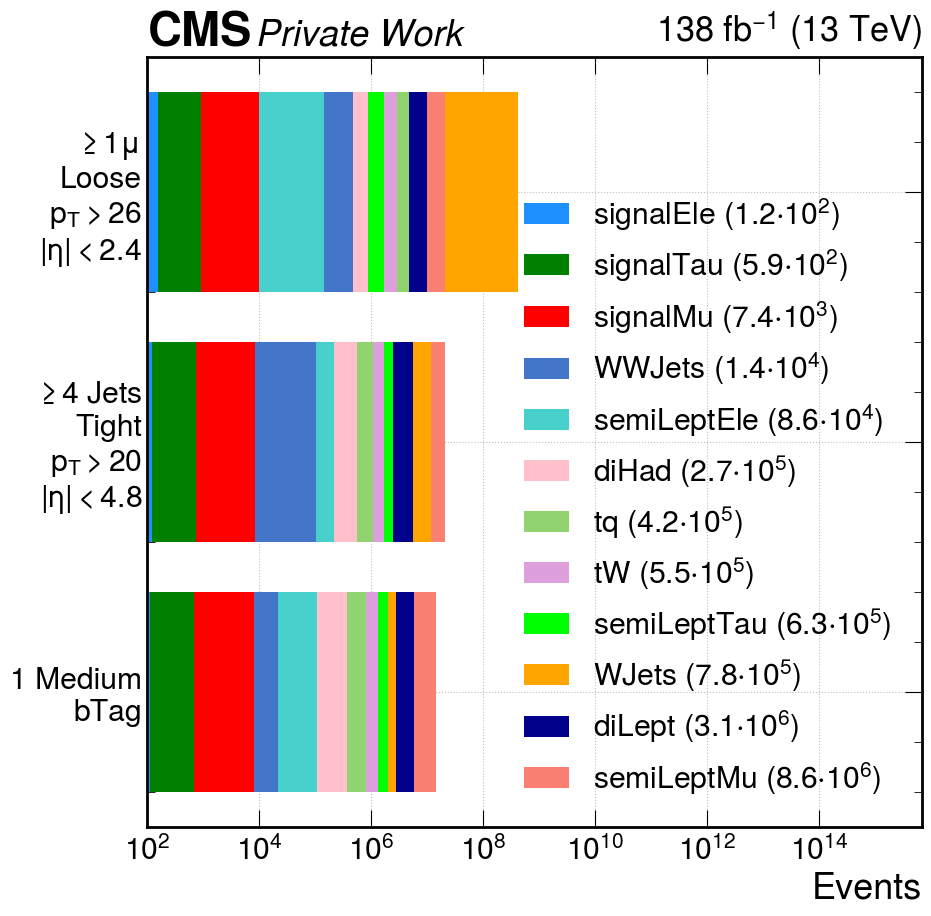
\includegraphics[width=\linewidth]{fig//chap07-selection/mu_selection.png}
         \caption{\textbf{Muons channel}}
     \end{subfigure}
     \vspace{0.5cm}
        \caption{Event number for each process for each cut. In the legend the final number of events for each process after the preselection is shown. The processes are ordered in their final event number.}
        \label{fig:event_selection}
\end{figure}
\newpage
\section{Neutrino reconstruction}
To fully reconstruct the kinematics of the event and to allow the reconstruction of the leptoninc decaying top quark, the longitudinal component of the neutrino was reconstructed exploiting the transverse momentum of the missing energy, its pseudorapidity, the lepton's four vector, and fixing the mass of the \PW boson to $m_W=80.385 \GeV$.
\begin{equation}
    (p^\mu_\nu+p^\mu_\ell)^2=m_W^2 
\end{equation}
The equation to solve for $p_z^{\nu}$ is a second order equation
\begin{equation*}
    p_z^\nu=\dfrac{p_z^\ell(m_W^2+2\vec{p}_T^{\:\ell} \cdot \vec{p}_T^{\:\nu})\pm\sqrt{(p_z^\ell)^2 (m_W^2+2\vec{p}_T^{\:\ell} \cdot \vec{p}_T^{\:\nu})^2-|p_T^\ell|^2[4(E_\ell p_T^\nu)^2-(m_W^2+2\vec{p}_T^{\:\ell} \cdot \vec{p}_T^{\:\ell})^2)]}}{2|p_T^\nu|^2}
\end{equation*}

The equation has two solutions, that can also be complex. If the equation has a complex solution the real part is taken but, if the equation allows two real solutions, we must choose one of them.\\
In \Fig{fig:nu_comparison} it is shown a comparison between the solution with the smaller magnitude, the solution with the greater magnitude, and the truth value of $p_z^\nu$ at the LHE level.\\
This study was performed using signal samples.


\begin{figure}[H]
    \centering
    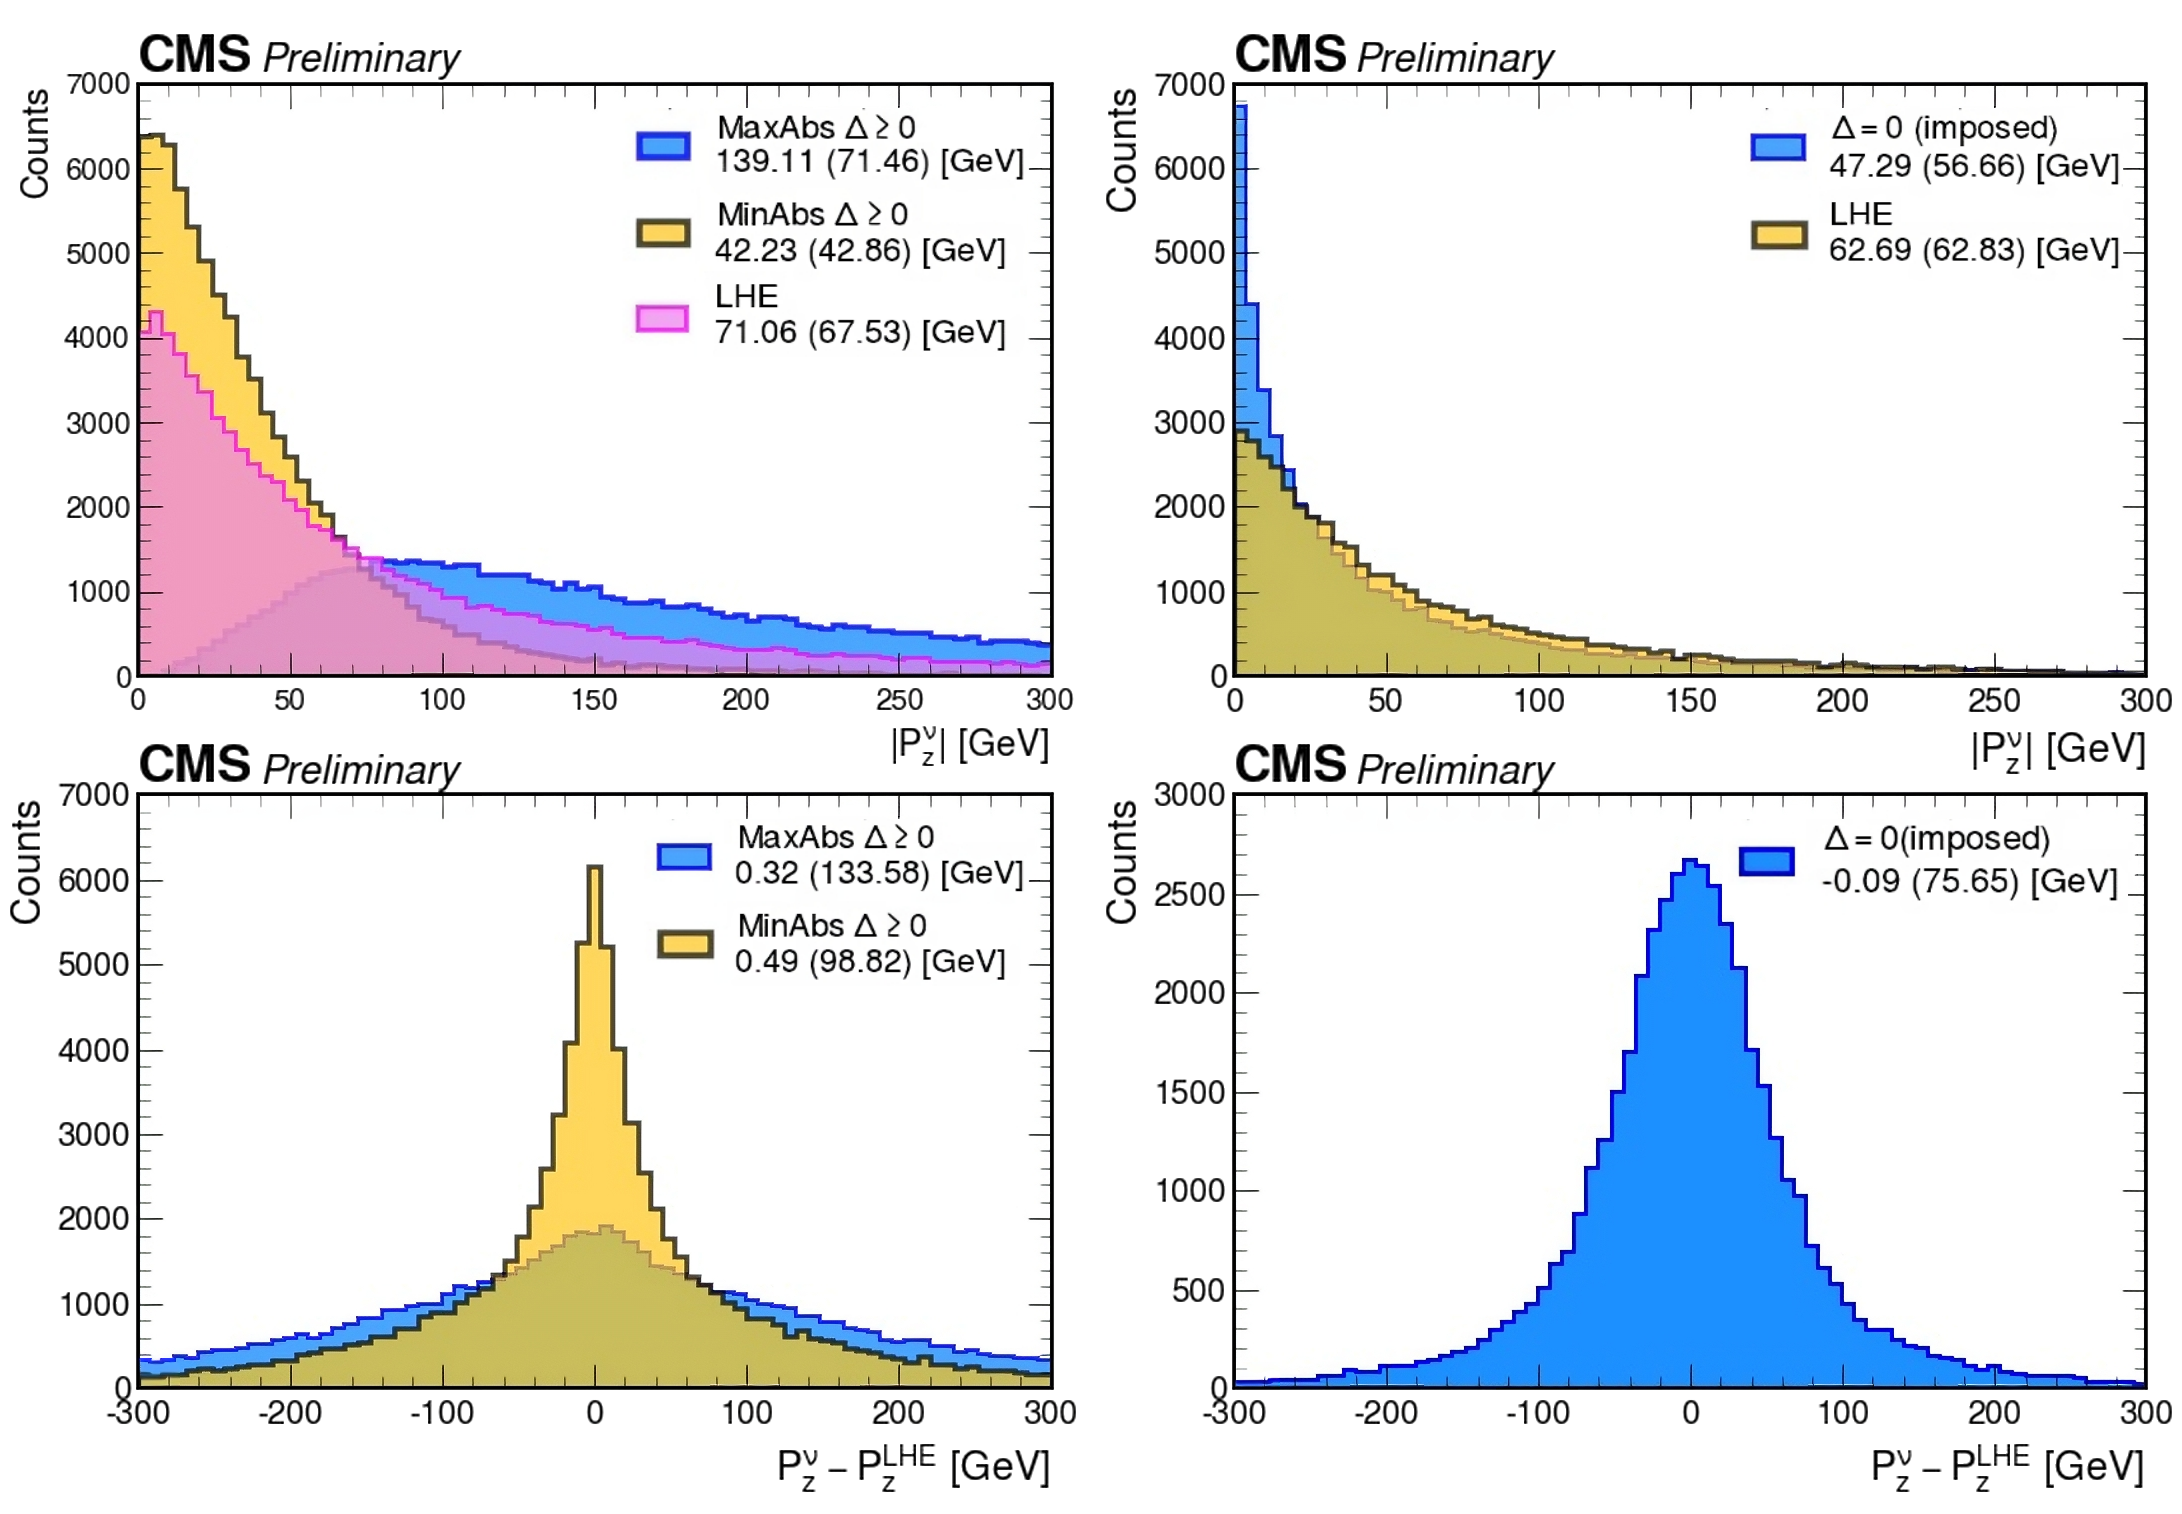
\includegraphics[width=1\linewidth]{fig//chap07-selection/Pznu_LHE_comparison.png}
    \caption{In the left panels there are the events that have two real solutions, while in the right panels the ones with the complex solutions of which only the real part is shown. In the top panel the distribution of the absolute value of the solutions and the LHE truth value are shown, while in the bottom panels, there are the distributions of the differences between the solutions and the LHE truth values. The $\Delta$ in the legend is the discriminant of the second-order equation. The distributions are in arbitrary units.}
    \label{fig:nu_comparison}
\end{figure}




The distribution of the solutions with the smaller absolute value is in better accordance with the truth value, so the strategy will be:\\
\begin{minipage}{\linewidth}
    \begin{minipage}{0.42\linewidth}

\begin{itemize}
    \item The solutions are complex: take the real part.
    \item There are two real solutions: take the smallest in the absolute value.
\end{itemize}

        Of course, in the complex solution case, if we consider only the real part, the chosen value will violate the W mass constraint, so, the invariant mass of the sum of the lepton and the reconstructed neutrino will not be $m_W$. In  \Fig{fig:LeptW_reco} the distribution of the leptonic W mass is shown.
    \end{minipage}
    \hfill
    \begin{minipage}{0.55\linewidth}
    \vspace{-0.2cm}
    \begin{figure}[H]
    \centering
    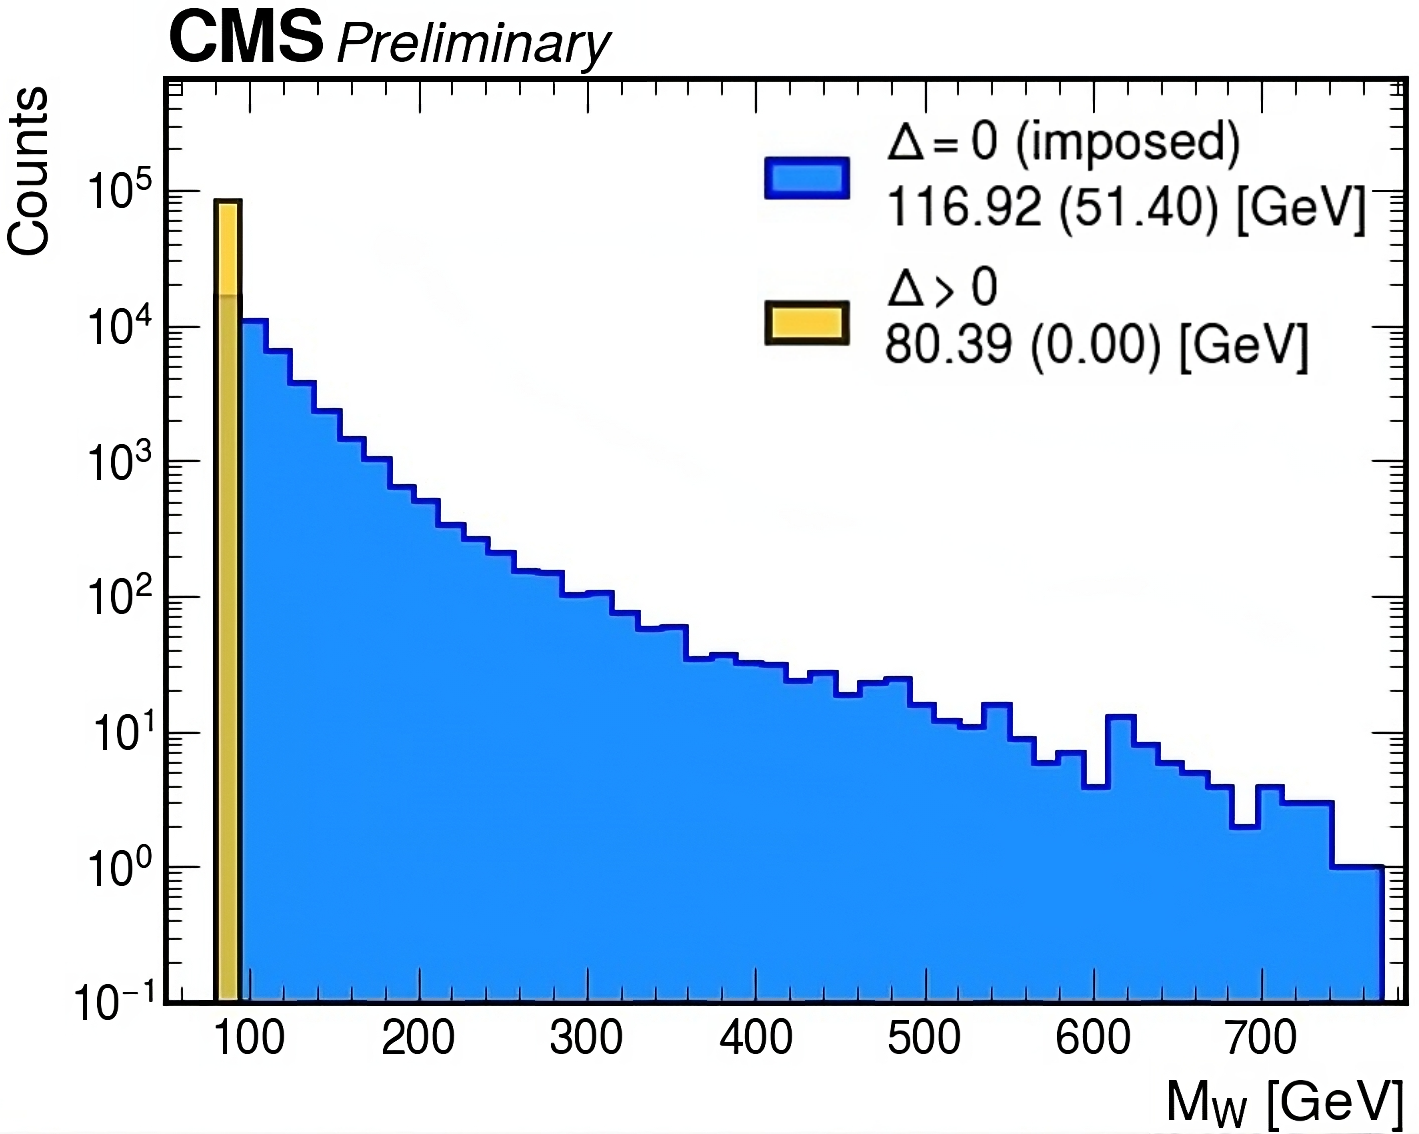
\includegraphics[width=\linewidth]{fig//chap07-selection/Wmass_reconstructed.png}
    \caption{Distribution of the reconstructed W mass in the real solution case and the complex solution case, taking only the real part.}
    \label{fig:LeptW_reco}
\end{figure}
        
    \end{minipage}

\end{minipage}

